\question[20] A dipole with dipole moment $p=qs=6.0\times10^{-30}\ \mathrm{C\cdot m}$ is centered at the origin. The two charges are separated by a distance $s=4.0\times10^{-12}$ m, with the positive charge lying on the positive side of the $x$ axis. What is the electric field $\vec{E}$ at the point $\vec{P}=<8.0\times 10^{-12},5.0\times10^{-12},0>$ m, which is neither on the dipole's parallel nor perpendicular axis? Be sure to express your answer as a vector with proper units.

\begin{center}
	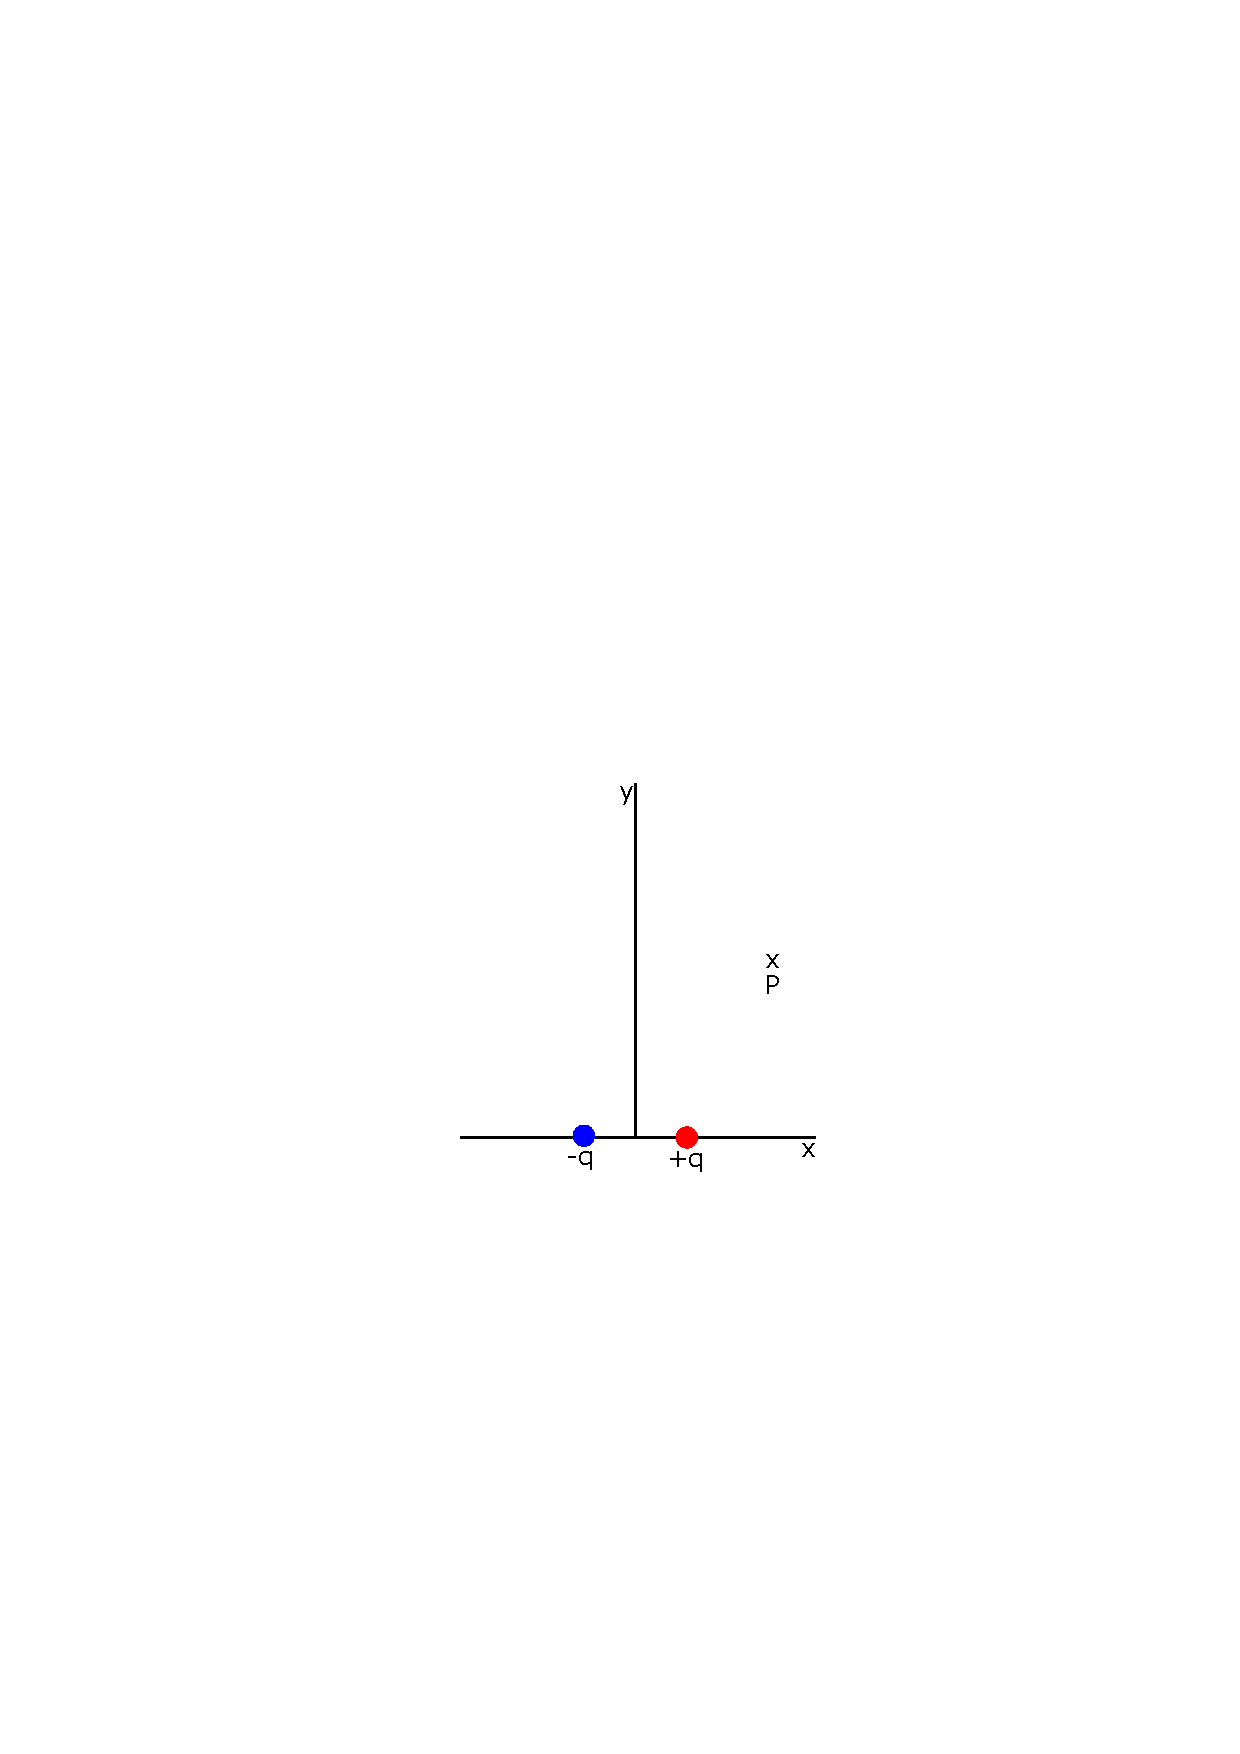
\includegraphics[width=.6\textwidth]{dipole}
\end{center}